\section{Frequentist Analysis}
\label{sec:frequentist}
% \todo{Marco -- section intro: one or two sentences on the frequentist approach (unbinned ML fit with \texttt{iminuit}, profile likelihood). Subsections below still use ``planned'' wording; rewrite in the past tense with the results.}

The frequentist analysis estimates \Araw by maximizing the extended unbinned likelihood of Eq.~\eqref{eq:likelihood}, i.e.\ the same model and the same window $[5100,5600]\,\MeV$ as the Bayesian analysis, with \texttt{iminuit}~\cite{iminuit}. The $B^+$ and $B^-$ samples were fitted simultaneously with \Araw as a fit parameter, and its uncertainty and the test of $A=0$ were derived from the profile likelihood, the other parameters being treated as nuisance parameters (Secs.~\ref{sec:freq_model}--\ref{sec:freq_ci}).


\subsection{Mass Model and Fit Strategy}
\label{sec:freq_model}
% The frequentist fit reuses the same physical mass model as the Bayesian analysis (Sec.~\ref{sec:bayes_model}), $f(m)=N_s\,S(m;\theta_s)+N_b\,B(m;\theta_b)$, estimated by unbinned maximum likelihood (\texttt{iminuit}~\cite{iminuit}, an interface to MINUIT~\cite{minuit}, with \texttt{iminuit.cost.ExtendedUnbinnedNLL}) rather than by Markov chain Monte Carlo (MCMC) sampling. The plan is to start from the same minimal shapes as the Bayesian baseline (Gaussian signal, exponential background) and increase model complexity only if the residuals justify it -- mirroring the Bayesian goodness-of-fit study (Sec.~\ref{sec:bayes_gof}), where a single exponential background is rejected by the data and a Crystal Ball signal improves the fit without moving $\Araw$. \todo{Marco -- fill in once the mass fit is run: final signal/background shapes chosen, fitted yields $N_s,N_b$, and any residual-based justification for departing from the minimal model.}

The frequentist fit uses the same physical mass model as the Bayesian analysis (Sec.~\ref{sec:bayes_model}, Eq.~\eqref{eq:mixture}) on the same window $[5100,5600]\,\MeV$: a Gaussian signal, with mean $\mu$ and width $\sigma$ shared by the two charges, and a double-exponential background with a shape and a yield of its own for each charge. The twelve parameters are the same as in the Bayesian fit, the two background yields being left free (equivalent to the pair $N_b$, $A_b$). They were estimated by maximizing the extended unbinned likelihood of Eq.~\eqref{eq:likelihood} through \texttt{iminuit.cost.ExtendedUnbinnedNLL}: the extended form is needed because the signal and background yields are fit parameters. The minimization started from a background description obtained independently of the signal, with an unbinned fit of the sidebands (the fit window without the region $[5200,5350]\,\MeV$) for each charge. The fit gives $N_s=15{,}327\pm133$ signal and $N_b=4{,}403\pm82$ background candidates, to be compared with the Bayesian posterior medians $15{,}328\pm133$ and $4404\pm82$ (Sec.~\ref{sec:bayes_posterior}).

The shapes were not tuned on the frequentist fit: the nominal model is the Bayesian one, and the alternatives are systematic variants (Sec.~\ref{sec:syst}). The nominal fit has $\chi^2/\mathrm{ndof}=160/88$ ($p=4.8\cdot 10^{-6}$) in $2\times50$ bins of $10\,\MeV$.
% A Crystal Ball signal with free tail parameters improves it to $407/386$ ($\Delta\chi^2=35$ for two more parameters, $p=0.22$), but moves \Araw by only $-0.0006$ (Table~\ref{tab:syst}), so the signal tails do not matter for the asymmetry and the Gaussian is kept as nominal.
The double exponential is required by the data: the background rises towards the lower edge of the window (Sec.~\ref{sec:data_mass}), and a single exponential is rejected ($\chi^2/\mathrm{ndof}=294/92$ ($p=5.7\cdot 10^{-23}$)), so for the systematic study only the double exponential is considered.
% The $p$-value depends on the binning: for the $10\,\MeV$ bins of the Bayesian study the nominal model has $\chi^2/\mathrm{ndof}=164.1/88$, an excess over the degrees of freedom of the same order as here ($76$ against $54$) but more significant, because the fluctuation of the $\chi^2$ grows only as $\sqrt{2\,\mathrm{ndof}}$.

\subsection{Separate vs.\ Simultaneous Fit}
\label{sec:freq_simfit}
% Two parametrizations are planned: a \emph{separate} fit of $B^+$ and $B^-$ independently, giving $N_s^+$ and $N_s^-$ from which $\Araw$ is computed post hoc, and a \emph{simultaneous} fit using the shared parametrization $N_s^+=N_s(1-A)/2$, $N_s^-=N_s(1+A)/2$ (the same parametrization already used on the Bayesian side, Sec.~\ref{sec:bayes_model}) that estimates $A$ directly as a fit parameter. Mass, resolution, and background-shape parameters are treated as nuisance parameters, profiled out when reporting the uncertainty on $A$. \todo{Marco -- report $\Araw$ from both parametrizations (should agree if the model is well-specified) and flag any disagreement as a modeling issue rather than a physics result.}

The asymmetry was estimated in two ways. In the \emph{simultaneous} fit the two charge samples share the signal parametrization $N_s^+=N_s(1-A)/2$, $N_s^-=N_s(1+A)/2$ (the same one used on the Bayesian side, Sec.~\ref{sec:bayes_model}) and the signal mean and width, so that $A$ is a parameter of the likelihood; mass, resolution and background-shape parameters are nuisance parameters, profiled out when reporting uncertainty on $A$. In the \emph{separate} fit each charge was fitted on its own with the same model and no parameter in common (seven free parameters per charge), and $\Araw=(N_s^--N_s^+)/(N_s^-+N_s^+)$ was computed afterwards from the two signal yields, with the uncertainty propagated from those of the yields, which are independent because the two samples are. The simultaneous fit gives $\Araw=-0.0441\pm0.0085$ and the separate fits $\Araw=-0.0442\pm0.0087$.

The two estimates agree, because sharing $\mu$ and $\sigma$ between $B^+$ and $B^-$, as expected for a particle and its antiparticle and a symmetric detector, is adequate.
Therefore the simultaneous fit, which estimates $A$ directly and gives the profile-likelihood interval of the next subsection, is taken as the nominal one.

\subsection{Profile Likelihood and Confidence Interval}
\label{sec:freq_ci}
% The profile likelihood ratio,
% \[
% q(A) = -2\log\frac{L(A,\hat{\hat\theta})}{L(\hat A,\hat\theta)},
% \]
% is used to derive a confidence interval on $A$ via Wilks' theorem~\cite{wilks}, and to test the null hypothesis $A=0$ -- the frequentist counterpart of the Bayesian Savage-Dickey test of Sec.~\ref{sec:bayes_factor}. \todo{Marco -- report the MLE $\hat A$, the 68\%/95\% profile-likelihood confidence intervals, and the $p$-value/significance against $A=0$; compare directly against the Bayesian credible interval of Sec.~\ref{sec:bayes_posterior} ($\Araw=-0.0443$, 68\% CI $[-0.0528,-0.0358]$) once available.}


The maximum-likelihood estimate is $\hat A=-0.0441$, with a Hesse uncertainty of $0.0085$, and the 68\% and 95\% Confidence Interval, CI, obtained with \texttt{MINOS}~\cite{minuit} are the following:
\begin{gather*}
\Araw = -0.0441, \\
68\%~\text{CI}~[-0.0526, -0.0356], \\ 95\%~\text{CI}~[-0.0607, -0.0275].
\end{gather*}
The uncertainties are statistical only; the systematic uncertainty is given in Sec.~\ref{sec:syst}.

The profile likelihood ratio,
\[
q(A) = -2\log\frac{L(A,\hat{\hat\theta})}{L(\hat A,\hat\theta)},
\]
where $\hat{\hat\theta}$ are the values of the other eleven parameters that maximize the likelihood at fixed $A$, was evaluated by re-minimizing them at each value of $A$ (the \texttt{mnprofile} of \texttt{iminuit}).
% By Wilks' theorem~\cite{wilks}, $q(A)$ follows a $\chi^2$ distribution with one degree of freedom at the true value of $A$, so the $68\%$ and $95\%$ confidence intervals are the sets of $A$ with $q(A)\leq1$ and $q(A)\leq3.84$ (the MINOS intervals~\cite{minuit}), which need not be symmetric.


For the null hypothesis $A=0$ it gives $q(0)\simeq27$, i.e.\ a $p$-value of $2.05\times10^{-7}$ corresponding to a significance of $5.20\sigma$: the hypothesis of no asymmetry is rejected. This is the frequentist counterpart of the Savage-Dickey test of Sec.~\ref{sec:bayes_factor}, where $A=0$ lies at $5.2$ posterior standard deviations.% and $BF_{01}\approx1.1\times10^{-4}$.
The two quantities do not measure the same thing (the $p$-value is not the probability of $H_0$, and the Bayes factor depends on the width of the prior), but they lead to the same conclusion.

The result agrees with the Bayesian one (Sec.~\ref{sec:bayes_posterior}: $\Araw=-0.0443$, $68\%$ CI $[-0.0528,-0.0358]$). This is expected: with flat priors and $\sim2\times10^4$ events the posterior is dominated by the likelihood and nearly Gaussian, so the credible and confidence intervals coincide numerically although their interpretations differ.

\subsection{Coverage of the Wilks Intervals}
\label{sec:freq_coverage}
% \todo{Marco -- coverage of the profile-likelihood interval on $A$ alone (1000 bootstrap replicas, nominal model, re-run notebook): $68.4\pm1.5\%$ for the 68.3\% interval; describe the procedure and compare with the Bayesian coverage of Sec.~\ref{sec:bayes_toymc}.}

Wilks' theorem~\cite{wilks} is an asymptotic result, so the coverage of the profile-likelihood interval on $A$ was checked directly on the data with a bootstrap. $1000$ replicas of the $19{,}731$ candidates of the fit window were drawn with replacement, which reproduces the statistical fluctuations of the sample, including those of the charge counts, and the nominal fit was repeated on each of them. The reference value of the asymmetry in the replicas is the best-fit value of the original data, $A_{\mathrm{true}}=-0.0441$. For each replica the statistic $q(A_{\mathrm{true}})$ was computed as the difference of $-2\log L$ between the fit with $A$ fixed to $A_{\mathrm{true}}$ and the fit with $A$ free and the other eleven parameters profiled. The $68\%$ interval of a replica contains $A_{\mathrm{true}}$ if and only if $q(A_{\mathrm{true}})\leq1$; replicas in which a fit did not converge were discarded.

The fraction of replicas with $q(A_{\mathrm{true}})\leq1$ is $68.4\pm1.5\%$ (binomial uncertainty), against the nominal $68.3\%$: the interval has the nominal coverage (Fig.~\ref{fig:freq_toys}). This agrees with the toy-MC check of the Bayesian credible interval (Sec.~\ref{sec:bayes_toymc}, $65.0\pm3.3\%$ for the $68\%$ interval); the two values differ by less than one standard deviation, and the uncertainty here is smaller because of the larger number of replicas ($1000$ against $200$). The two checks are not equivalent. The Bayesian pseudo-datasets are generated from the fitted model, which makes that check a closure test, while the replicas here are resampled from the data and therefore carry the features of the spectrum that the model does not describe, such as the shape of the signal tails (Sec.~\ref{sec:bayes_gof}). %That the nominal coverage is obtained nevertheless suggests that the imperfect description of the spectrum does not invalidate the profile-likelihood interval of $A$.

\begin{figure}[h]
\centering
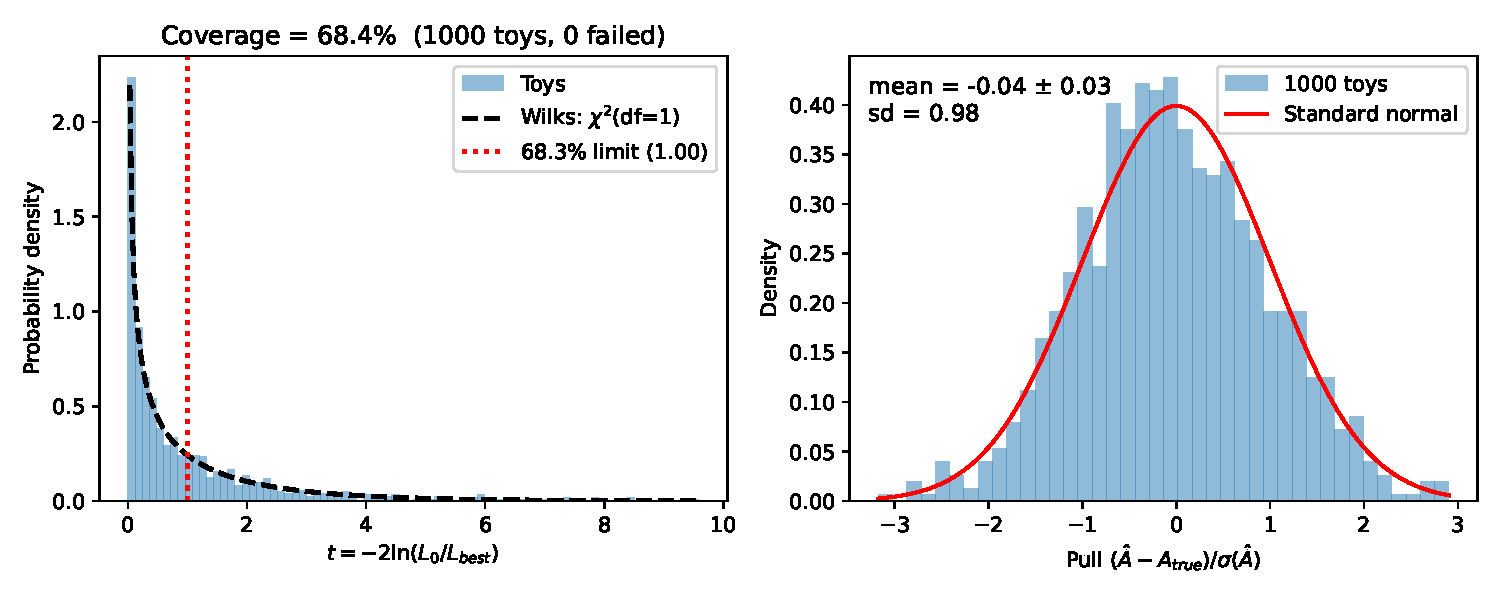
\includegraphics[width=\columnwidth]{figures/frequentist_wilks_coverage.pdf}
\caption{Coverage check, 1000 toys. Left: the statistics $q(A_{\mathrm{true}})$ following a $\chi^2_{dof=1}$ distribution as expected from Wilks theorem. Right: pulls $(\hat A-A_{\mathrm{true}})/\sigma(\hat A)$, with $\hat A$ and $\sigma(\hat A)$ the fit results of each toy, compared with a standard normal. }
\label{fig:freq_toys}
\end{figure}

\subsection{Systematic Uncertainties and Stability Checks}
\label{sec:freq_syst}
While the systematic uncertainties study is shared with the Bayesian approach -- and discussed in detail in Sec.~\ref{sec:syst} -- three specific stability checks were performed within the frequentist one, to evaluate the robustness of the fitted raw asymmetry $\Araw$. Each test consists of a two-dimensional grid scan in which two selection or fit parameters are varied simultaneously, performing a simultaneous fit with the nominal double-exponential background model at each point and observing the stability of $\Araw$.

\begin{enumerate}[leftmargin=*]
    \item \textbf{Fit Window Scan:} The lower and upper boundaries of the invariant mass fit window, nominally set to $[5100, 5600]\,\MeV$, were scanned over the ranges $[5000, 5200]\,\MeV$ and $[5350, 6100]\,\MeV$, respectively, with a 50 \MeV step. This test evaluates the sensitivity of $\Araw$ to the exponential background parametrization, and is useful to choose the nominal window: too small or too asymmetric fit window produces unstable fit, due to worse background estimation.

    \item \textbf{Signal Region Scan:} Changing the extremes of the signal region not significant fluctation in $\Araw$ are observed, suggesting that the sideband preliminar fit could be avoided.

    \item \textbf{Particle Identification Cut Scan:} The preselection cuts on the final-state kaon PID likelihoods (\texttt{ProbK} and \texttt{ProbPi}) were varied simultaneously towards a better kaon purity (larger than $0.5$ for kaons, smaller than $0.5$ for pions). This influences significantly the $\Araw$ estimation, but always within the $68\%$ CI, confirming the cut selection as reasonable.
\end{enumerate}

Across all scan configurations, the maximum observed variation in $\Araw$ remains below the statistical uncertainty ($\Delta \Araw < \sigma_{\mathrm{stat}}$), demonstrating the stability of the nominal fit result.
